\section{Modello di predizione}
\subsection{Introduzione}
Uno degli obiettivi principali di questo progetto è stato quello di sviluppare un modello di machine learning capace di predire l'esito delle partite NBA. Questo rappresenta una sfida ambiziosa che richiede un'analisi approfondita delle statistiche delle squadre e l'applicazione di avanzate tecniche di ML. Il dataset utilizzato comprende un array di statistiche per ciascuna squadra, sia per la squadra di casa che per quella in trasferta.

Sono stati testati sette differenti modelli sul set di training: Multi-Layer Perceptron (MLP), Random Forest, Support Vector Machine (SVM), XGBoost, Regressione Lineare, Modello Bayesiano e K-Nearest Neighbors (KNN).


Per sviluppare un modello competitivo rispetto alle soluzioni attualmente disponibili sul mercato, è stato inizialmente affrontato il problema come una questione di classificazione, utilizzando un MLP. Dato che i risultati ottenuti erano promettenti, sono state poi esplorate ulteriori possibilità per migliorare le prestazioni del modello. Di conseguenza, è stato convertito il problema di classificazione in un problema di regressione, con l'obiettivo di prevedere non solo l'esito (vittoria o sconfitta) ma anche il margine di punti con cui una squadra vince o perde.

L'approccio di regressione offre un livello di dettaglio superiore, consentendo non solo di determinare il vincitore della partita, ma anche di fornire una stima più precisa delle prestazioni delle squadre. Questa dualità di approccio, classificazione e regressione, ci permette di ottenere un modello robusto e versatile, in grado di adattarsi a diverse esigenze di predizione nel contesto delle partite NBA.

In sintesi, il progetto si articola in due fasi principali:
\begin{enumerate}
    \item Creazione e valutazione di un modello di classificazione tramite MLP.
    \item Espansione del modello in un contesto di regressione per migliorare la precisione delle predizioni.
\end{enumerate}

I risultati ottenuti dalle varie sperimentazioni con i diversi modelli saranno discussi nelle sezioni successive, evidenziando i vantaggi e le limitazioni di ciascun approccio.

\subsection{Il Dataset}

I dati utilizzati per addestrare e testare i modelli sono stati raccolti da una vasta gamma di statistiche presenti nel Database di NBA.com. Per la scelta e la selezione di queste statistiche sono state prese in considerazione numerose risorse online tra cui ad esempio il paper "Which NBA Statistics Actually Translate to Wins" di Chinmay Vayda. Queste varie ricerche ci hanno così permesso di trovare quelle che a nostro avviso solo le statistiche più rilevanti per la predizione delle partite NBA.\newline
\newline
\texttt{['home\_team','away\_team','game\_id','season','date','pts\_H','pts\_A','winner','playoff', \newline
'fg\_pct\_A','fg3\_pct\_A','ft\_pct\_A','reb\_A','tot\_ast\_A','tot\_tov\_A','tot\_stl\_A',\newline
'tot\_blk\_A','ts\_pct\_A','w\_pct\_A','w\_pct\_last\_5\_games\_A','fg\_pct\_H','fg3\_pct\_H',\newline
'ft\_pct\_H','reb\_H','tot\_ast\_H','tot\_tov\_H','tot\_stl\_H','tot\_blk\_H', \newline
'ts\_pct\_H','w\_pct\_H','w\_pct\_last\_5\_games\_H','off\_rating\_A','def\_rating\_A',\newline
'off\_rating\_H','def\_rating\_H','lineup\_efficiency\_A','lineup\_efficiency\_H',\newline
'referee\_name','referee\_id']}\\
\\
Questo è il Dataset da noi creato ed ottenuto tramite la \texttt{nba\_api}. Risulta essere un dataset molto ampio e completo, che è stato poi ridotto e lavorato in fase di preprocessing e fine-tuning dei vari modelli.

\subsection{Il Modello di Classificazione}

\subsubsection{MLP}

\paragraph{Introduzione al MLP}
Il Multi-Layer Perceptron (MLP) è una classe di reti neurali artificiali ampiamente utilizzata nei problemi di classificazione e regressione. Un MLP è composto da uno strato di input, uno o più strati nascosti e uno strato di output. Ogni nodo (o neurone) in uno strato è connesso a ciascun nodo nel successivo strato, rendendolo un tipo di rete completamente connessa. I MLP utilizzano la retropropagazione per allenare il modello, aggiornando i pesi dei neuroni in base all'errore commesso nelle predizioni.
\begin{figure}[H]
    \centering
    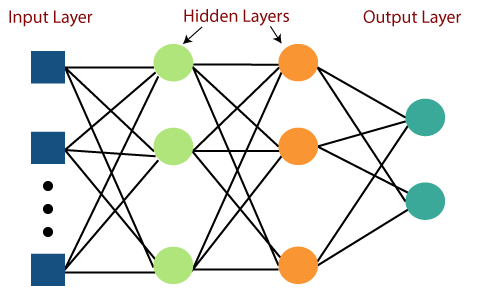
\includegraphics[width=0.3\linewidth]{img/multi-layer-perceptron-in-tensorflow.png}
    \caption{Multi-Layer Perceptron}
    \label{fig:enter-label}
\end{figure}

\paragraph{Sviluppo del Modello}
L'idea iniziale è stata quella di creare un MLP per risolvere il problema di classificazione. Il primo passo è stato quello di effettuare il preprocessing dei dati, eliminando tutte le informazioni non necessarie per l'allenamento della rete o eliminando informazioni che rendevano il modello meno accurato( e dunque meno performante). In particolare, sono stati rimossi i seguenti campi: \newline
\texttt{['pts\_H', 'pts\_A', 'referee\_id', 'winner', 'home\_team', 'away\_team', 'referee\_name', \newline
'season', 'date']}

Inoltre, prima di poter utilizzare il vettore finale, composto dunque dalle statistiche delle due squadre, per allenare il nostro modello, è stato necessario preprocessarlo. È stato quindi usato il \texttt{MinMaxScaler}, ovvero un algoritmo che garantisce che i valori fossero compresi tra -1 e 1, il che ha portato notevoli miglioramenti sia in termini di accuracy del modello sia in termini di performance della rete.

\paragraph{Struttura del Modello}
Il modello di machine learning è stato quindi costruito utilizzando tre strati \texttt{Dense}, ovvero strati fortemente connessi in grado di apprendere dai dati in input per ottenere un preciso output. La rete neurale ottenuta è stata quindi addestrata, come consuetudine, utilizzando l'80\% del Dataset suddiviso il Train Set e Validation Set.
Per migliorare ulteriormente il modello è stato eseguito un processo di fine-tuning manuale per massimizzare l'accuratezza.

\begin{figure}[H]
    \centering
    \begin{minipage}[b]{0.45\linewidth}
        \centering
        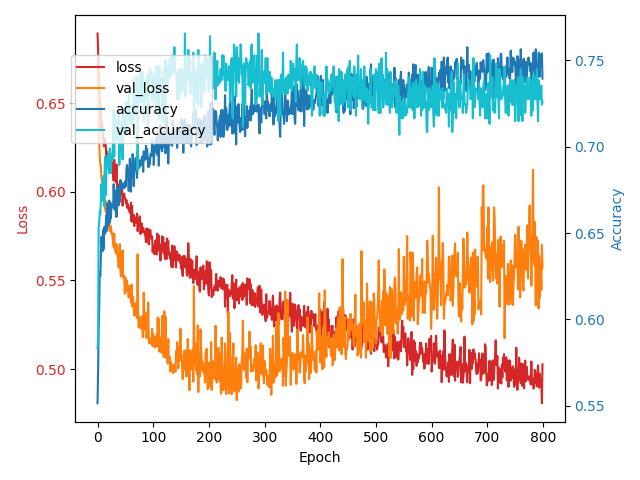
\includegraphics[width=\linewidth]{img/final800.png}
        \caption{Pre Fine-Tuning e Overfitting}
        \label{fig:first_label}
    \end{minipage}
    \hspace{0.05\linewidth}
    \begin{minipage}[b]{0.45\linewidth}
        \centering
        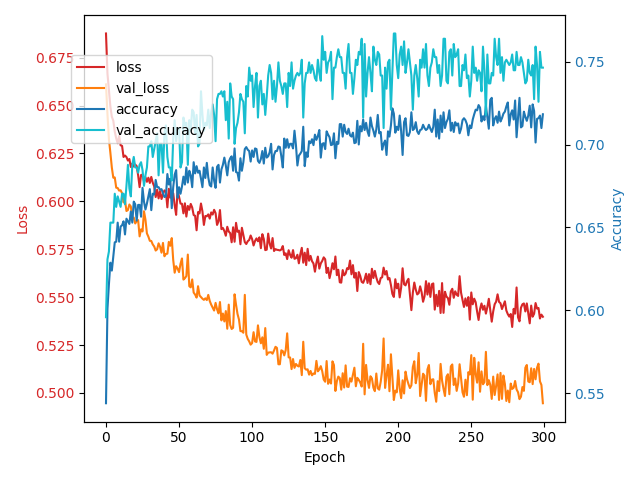
\includegraphics[width=\linewidth]{img/final_mlp.png}
        \caption{Post Fine-Tuning}
        \label{fig:second_label}
    \end{minipage}
\end{figure}

Inizialmente, è stato utilizzato un \textit{batch size} di 16 e sono state impostate 800 epoche per monitorare la funzione di \textit{loss} e identificare il punto di \textit{overfitting} del modello. Attraverso questo processo, è stato determinato che i parametri ideali per l'allenamento erano 300 epoche e un \textit{batch size} di 32.

\paragraph{Risultati}
Prima di poter analizzare questo risultato occorre precisare che l'accuracy fornita dai modelli citati online risulta essere tra il 62\% ed il 66\%. In relazione a ciò è presente un interessante articolo, redatto dalla Bryant University, nel quale presentano il loro modello che possiede una accuracy del 65\%.

In quest'ottica è possibile dire che il nostro modello finale ha ottenuto un'accuratezza estremamente competitiva, ottenendo una accuracy del 69,92\%, dimostrando così la validità dell'approccio MLP nel contesto della classificazione delle partite NBA. Questi risultati indicano che il nostro modello è in grado di fornire predizioni accurate (7 volte su 10) sulla vittoria o sconfitta delle squadre, basandosi sulle statistiche pre-partita.

In sintesi, l'implementazione del MLP come modello di classificazione ha fornito una solida base per ulteriori miglioramenti e ottimizzazioni, consentendo di esplorare ulteriori tecniche e modelli per migliorare le capacità predittive.
\begin{lstlisting}
Results MLP:
    Loss: 0.5629295706748962
    Accuracy: 0.6992385983467102
\end{lstlisting}


\subsection{I Modelli di Regressione}
Come anticipato, il problema di classificazione è stato convertito in un problema di regressione, in modo da testare nuovi approcci e verificare se il modello ottenuto potesse essere ulteriormente migliorato.
Tutti i modelli analizzati in questa sezione sono stati prima ottimizzati utilizzando una \texttt{GridSearch} per ottenere la combinazione ideale di iperparametri per ciascun modello.\\
Di seguito, verranno quindi analizzati i vari modelli e i risultati ottenuti, in ordine crescente di accuracy fornita.

\subsubsection{Analisi delle metriche}
Nel valutare le prestazioni del modello di regressione per la predizione dei risultati delle partite NBA, sono stati utilizzati diversi indicatori chiave di errore e precisione.

\begin{itemize}
    \item \textbf{Mean Absolute Error (MAE):} Il MAE misura la deviazione media tra le predizioni del modello e i valori reali. Nel nostro caso, il MAE indica dunque l'errore medio tra la differenza di punti predetti dal modello e i risultati reali delle partite.

    \item \textbf{Mean Squared Error (MSE):} Il MSE misura la media dei quadrati delle differenze tra predizioni e valori reali. Il MSE evidenzia dunque una variabilità nelle differenze tra predizioni e valori reali rispetto al MAE.

    \item \textbf{Root Mean Squared Error (RMSE):} Il RMSE è la radice quadrata del MSE ed è espresso nelle stesse unità della variabile target. Nel nostro caso, il RMSE indica che in media le predizioni del modello hanno un errore di una certa quantità di punti rispetto ai risultati reali.

    \item \textbf{Sign Accuracy:} La Sign Accuracy rappresenta la precisione del modello nel predire correttamente la direzione (positiva o negativa) delle differenze tra predizioni e valori reali. Questa metrica misura se il segno tra la differenza dei punti predetti e quella reale è concorde, in modo da prevedere quindi il vincitore di una partita indipendentemente dalla differenza dei punti.
\end{itemize}

Queste metriche forniscono una valutazione completa delle performance del modello di regressione, evidenziando sia l'errore medio delle predizioni che la sua capacità di predire correttamente l'esito delle partite NBA. Il confronto tra MAE, MSE e RMSE fornisce una panoramica dell'accuratezza delle predizioni a diversi livelli di dettaglio, mentre la Sign Accuracy fornisce una misura della precisione nella classificazione della direzione delle differenze.

\subsubsection{KNN}

Il K-Nearest Neighbors (KNN) è un algoritmo di machine learning utilizzato per problemi di classificazione e regressione. Nel contesto della regressione, KNN prevede il valore di una variabile target basandosi sui valori medi dei \textit{k} vicini più prossimi nel dataset di addestramento. La vicinanza tra i punti dati è solitamente calcolata tramite una metrica di distanza, come la distanza euclidea. KNN è semplice da implementare e interpretare, ma può essere computazionalmente costoso per dataset di grandi dimensioni.


Il modello KNN è stato valutato utilizzando diverse metriche di errore, ottenendo i seguenti risultati:
\begin{lstlisting}
    Mean Absolute Error (MAE): 11.620278833967047
    Mean Squared Error (MSE): 215.66732572877058
    Root Mean Squared Error (RMSE): 14.6856162869922
    Sign Accuracy: 0.6172370088719898
\end{lstlisting}
Il modello ha raggiunto un'accuratezza del 61,72\%.

Sono stati estratti 10 match casuali dal test set per valutare le prestazioni del modello, ottenendo i seguenti risultati:
\begin{figure}[H]
    \centering
    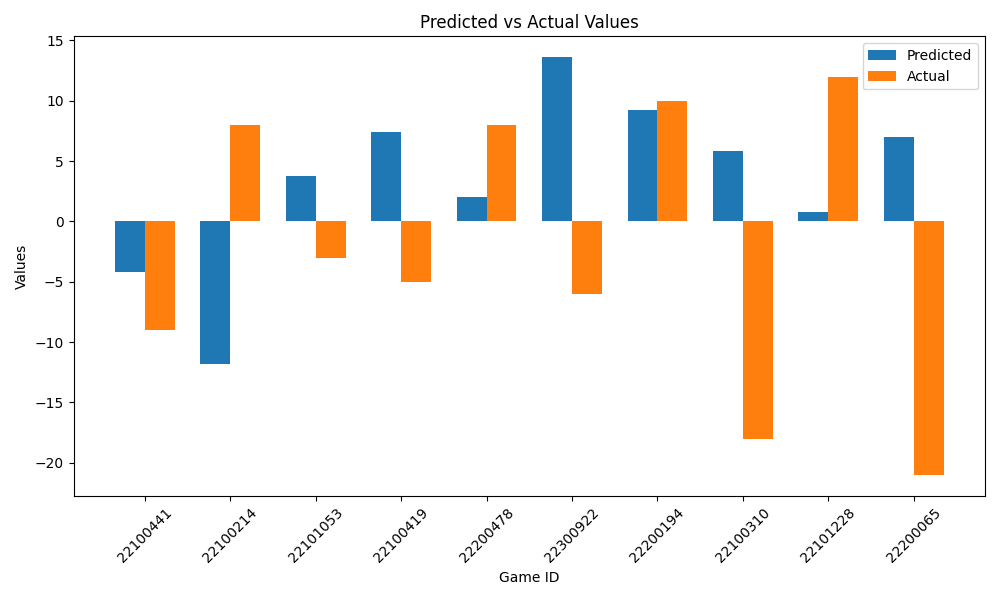
\includegraphics[width=0.7\linewidth]{img/knn_istogramma.png}
    \caption{Comparazione differenza punti predetti rispetto a reali in KNN}
    \label{fig:enter-label}
\end{figure}

\subsubsection{SVM}

Il modello SVM ha mostrato un'accuratezza migliore rispetto ad altri approcci. SVM (Support Vector Machine) è un algoritmo di apprendimento supervisionato utilizzato per la classificazione e la regressione. Esso cerca di trovare il miglior iperpiano o separatore tra i punti dei dati delle diverse classi. Nella figura sottostante è rappresentato un esempio di SVM con due classi.

Questo modello ha ottenuto i seguenti risultati nei test:

\begin{lstlisting}
    Mean Absolute Error (MAE): 10.360566704859455
    Mean Squared Error (MSE): 173.73226432418772
    Root Mean Squared Error (RMSE): 13.18075355676555
    Sign Accuracy: 0.6806083650190115
\end{lstlisting}

Il modello ha raggiunto un'accuratezza del 68.06\%. Inoltre, sono stati estratti 10 match casuali dal set di test per valutare ulteriormente le prestazioni del modello:

\begin{figure}[H]
    \centering
    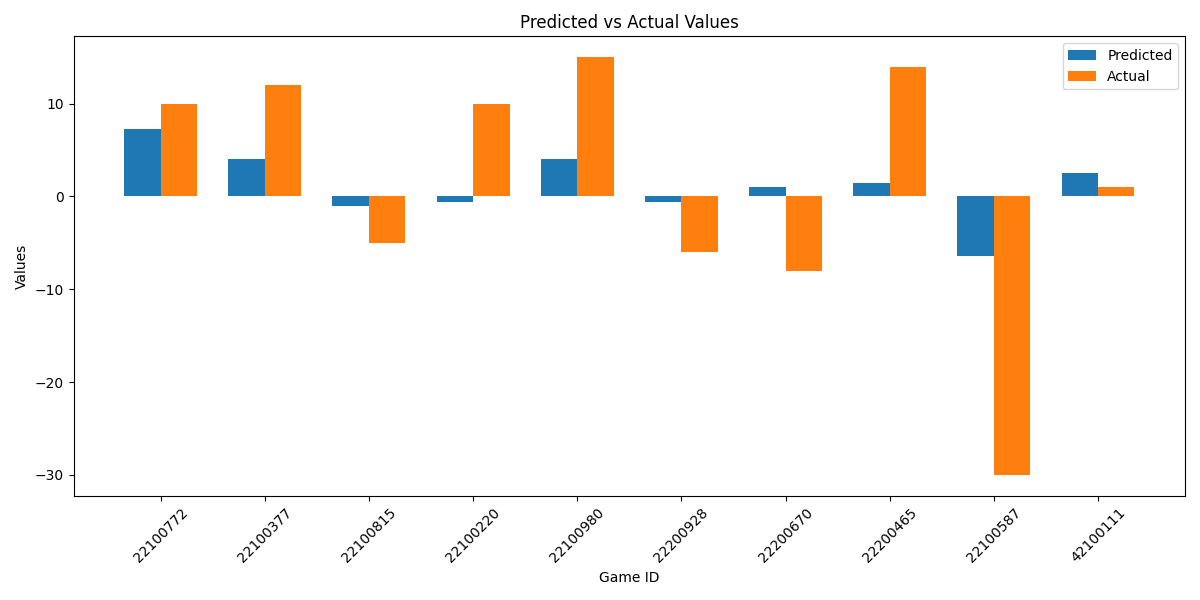
\includegraphics[width=0.7\linewidth]{img/svm.png}
    \caption{Comparazione differenza punti predetti rispetto a reali in SVM}
    \label{fig:enter-label}
\end{figure}

Questi risultati dimostrano che il modello SVM ha una buona capacità predittiva per l'esito delle partite NBA, con un'ottima precisione e una buona gestione della variazione nei dati di test.

\subsubsection{Random Forest}

Il Random Forest è un metodo di apprendimento \textit{ensemble} utilizzato per la classificazione e la regressione. Esso costruisce diversi alberi decisionali e li combina per ottenere previsioni più accurate. In un random forest, solo un sottoinsieme delle caratteristiche è considerato dall'algoritmo per dividere un nodo. Il modello classificherà anche l'importanza di ciascuna caratteristica nel prendere la decisione finale. Nella figura sottostante c'è un esempio di random forest con due alberi.

Questo modello ha ottenuto risultati soddisfacenti nei test, come mostrato di seguito:

\begin{lstlisting}
    Mean Absolute Error (MAE): 9.944223032615545
    Mean Squared Error (MSE): 159.938928930258
    Root Mean Squared Error (RMSE): 12.646696364278617
    Sign Accuracy: 0.6958174904942965
\end{lstlisting}

Il modello ha raggiunto un'accuratezza del 69.58\%. Inoltre, sono stati estratti 10 match casuali dal set di test per valutare ulteriormente le prestazioni del modello:

\begin{figure}[H]
    \centering
    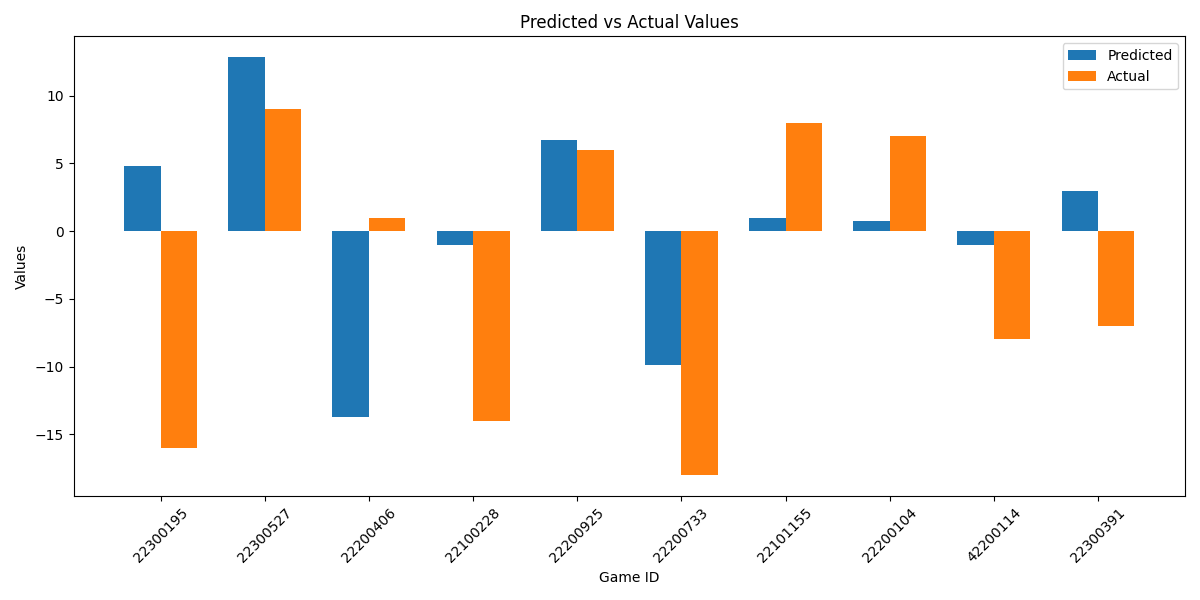
\includegraphics[width=0.7\linewidth]{img/random_forest_istogramma.png}
    \caption{Comparazione differenza punti predetti rispetto a reali in Random Forest}
    \label{fig:enter-label}
\end{figure}

Questi risultati indicano che anche il modello Random Forest si è dimostrato essere efficace nel predire l'esito delle partite NBA, con un'elevata accuratezza e una buona capacità di generalizzazione su nuovi dati di test.

\subsubsection{XGBoost}

XGBoost è un algoritmo di boosting estremamente popolare e efficace utilizzato per la classificazione e la regressione. Utilizza un insieme di alberi decisionali deboli, chiamati "weak learners", e li combina per migliorare progressivamente le prestazioni del modello.

Questo modello ha ottenuto i seguenti risultati nei test:

\begin{lstlisting}
    Mean Absolute Error (MAE): 9.6111730557072
    Mean Squared Error (MSE): 149.89162676035912
    Root Mean Squared Error (RMSE): 12.243023595515902
    Sign Accuracy: 0.7046894803548795
\end{lstlisting}

Il modello ha raggiunto un'accuratezza del 70.47\%. Inoltre, sono stati estratti 10 match casuali dal set di test per valutare ulteriormente le prestazioni del modello:

\begin{figure}[H]
    \centering
    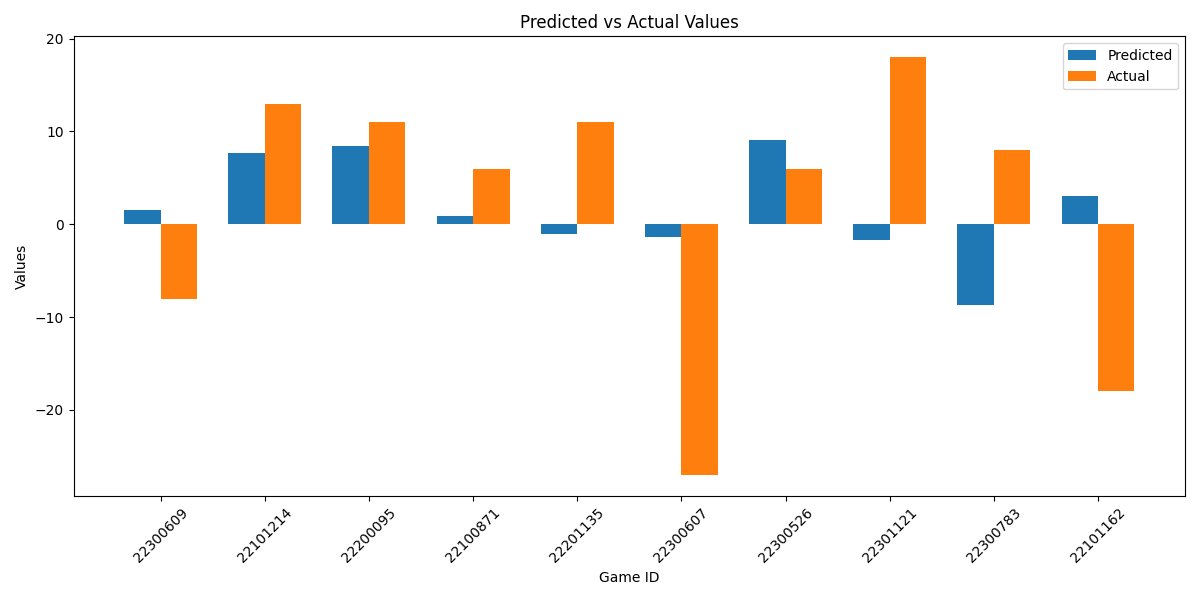
\includegraphics[width=0.7\linewidth]{img/xgboost_istogramma.png}
    \caption{Comparazione differenza punti predetti rispetto a reali in XGBoost}
    \label{fig:enter-label}
\end{figure}

Questi risultati indicano che il modello XGBoost risulta essere altamente efficace nel predire l'esito delle partite NBA. L'utilizzo di boosting ha permesso al modello di migliorare costantemente la precisione delle predizioni, rendendolo infatti una scelta potente per problemi complessi, come quello delle previsioni sportive.


\subsubsection{Bayesian}

Il modello Bayesian utilizza l'inferenza Bayesiana per stimare parametri incogniti. È particolarmente utile quando si hanno dati limitati e si desidera incorporare conoscenze pregresse o informative nel modello.

Questo modello ha ottenuto i seguenti risultati nei test:

\begin{lstlisting}
    Mean Absolute Error (MAE): 9.684169695449112
    Mean Squared Error (MSE): 151.8468062429373
    Root Mean Squared Error (RMSE): 12.322613612498662
    Sign Accuracy: 0.7072243346007605
\end{lstlisting}

Il modello ha raggiunto un'accuratezza del 70.72\%. Inoltre, sono stati estratti 10 match casuali dal set di test per valutare ulteriormente le prestazioni del modello:

\begin{figure}[H]
    \centering
    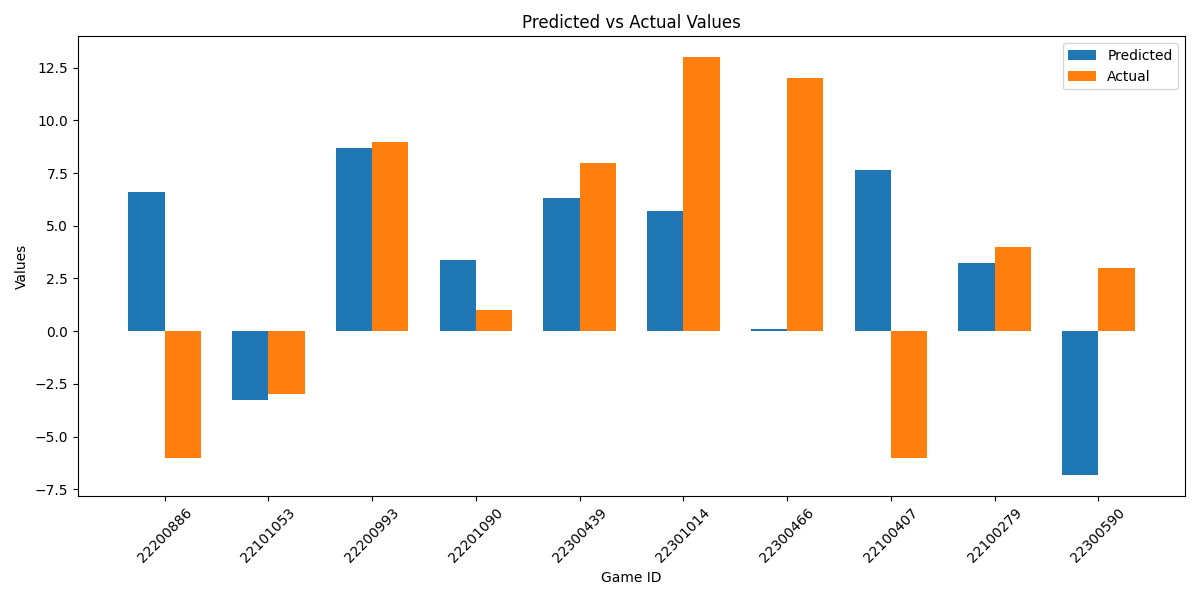
\includegraphics[width=0.7\linewidth]{img/bayesian_istogramma.png}
    \caption{Comparazione differenza punti predetti rispetto a reali in Bayesian}
    \label{fig:enter-label}
\end{figure}

Questi risultati validano la qualità del modello Bayesian, che ha mostrato una robusta gestione dell'incertezza nei dati di test. L'approccio basato sull'inferenza Bayesiana ha permesso al modello di integrare informazioni a priori con i dati osservati, migliorando così le performance complessive delle previsioni.


\subsubsection{Linear Regression}

La regressione lineare è un modello di machine learning che cerca di trovare la relazione lineare migliore tra una variabile dipendente (target) e una o più variabili indipendenti (features). È un metodo semplice ma potente per la predizione numerica.

Questo modello ha ottenuto i seguenti risultati nei test:

\begin{lstlisting}
    Mean Absolute Error (MAE): 9.673524553632301
    Mean Squared Error (MSE): 151.58868540348476
    Root Mean Squared Error (RMSE): 12.312135696274824
    Sign Accuracy: 0.7135614702154626
\end{lstlisting}

Il modello ha raggiunto un'accuratezza del 71.36\%. Inoltre, sono stati estratti 10 match casuali dal set di test per valutare ulteriormente le prestazioni del modello:

\begin{figure}[H]
    \centering
    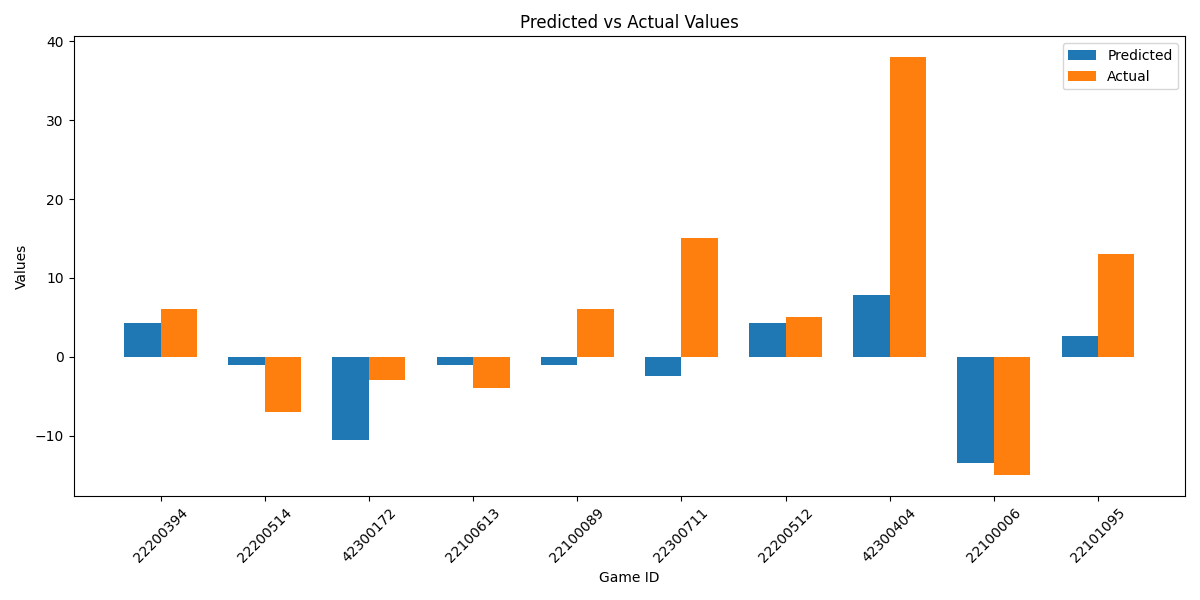
\includegraphics[width=0.7\linewidth]{img/linear_regression_istogramma.png}
    \caption{Comparazione differenza punti predetti rispetto a reali in Linear Regression}
    \label{fig:enter-label}
\end{figure}

Questi risultati indicano che il modello di Regressione Lineare ha fornito la migliore capacità predittiva, con un'efficace modellazione della relazione lineare tra le variabili di input e il target. La semplicità e la trasparenza della regressione lineare lo rendono un buon punto di partenza per esplorare i modelli di previsione numerica nelle analisi sportive.


\subsection{I Risultati}
È dunque possibile ora analizzare i dati in maniera unitaria e completa. Per effettuare ciò occorre suddifidere l'analisi dei risultati in due distinte sezioni, una per analizzare i risultati inerenti al problema di classificazione: Vittoria o Sconfitta, ed un'altra per analizzare i risultati del problema di regressione.

Inerentemente al problema di classificazione, per gli algoritmi di regressione è stata creata una nuova metrica fittizia denominata sign accuracy che ci ha permesso di convertire il problema di regressione in classificazione.
Comparando così le varie sign accuracy ottenute con i vari algoritmi, otteniamo il seguente risultato.
\begin{figure}[H]
    \centering
    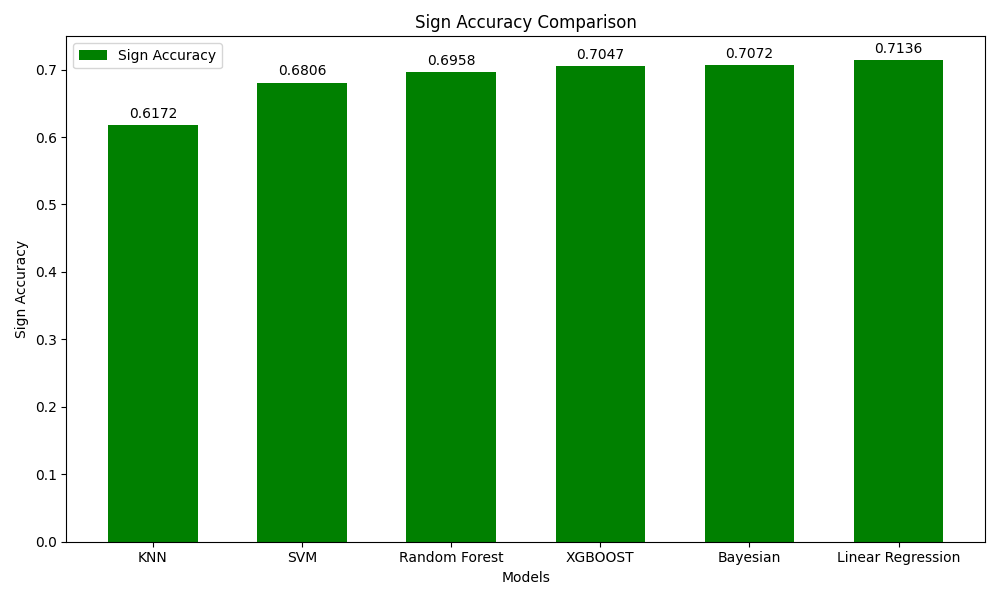
\includegraphics[width=0.7\linewidth]{img/sign_accuracy.png}
    \caption{Sign accuracy a confronto}
    \label{fig:enter-label}
\end{figure}

È possibile notare che l'algoritmo che ci fornisce una sign accuracy migliore è il Linear Regression che totalizza una precisione del 71,36\%. Questo è poi seguito dal Bayesian Regressor con 70,72\% e dal XGBoost Regressor con 70,46\%.
Questi algoritmi sono quindi riusciti ad ottenere, a parità di input, un risultato migliore anche del modello MLP definito inizialmente.
In ultima posizione, vediamo come il K-Nearest Neighbor abbia le prestazioni peggiori. 
\newline

Concentrandoci ora sull'analisi del problema di regressione e dunque sull'analisi della differenza tra i punti predetti ed i punti reali otteniamo risultati leggermente diversi.
A tal proposito è stata messa a confronto la metrica \texttt{Mean Absolute Error}, che fornisce informazioni riguardanti l'errore medio dei vari modelli creati.
Confrontando quindi questa metrica sono stati ottenuti i seguenti risultati.
\begin{figure}[H]
    \centering
    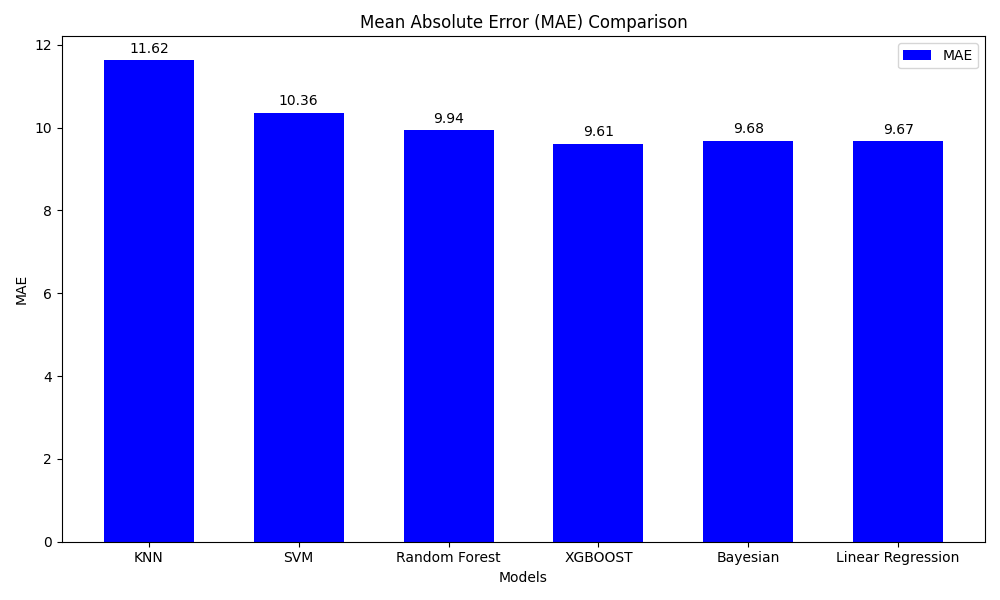
\includegraphics[width=0.7\linewidth]{img/mae_a_confronto.png}
    \caption{Caption}
    \label{fig:enter-label}
\end{figure}

L'algoritmo più performante in termini di regressione risulta essere XGBoost con 9,61 punti di scarto medio, seguito poi dalla Linear Regression con 9,67 punti e dal Bayesian con 9,68.
Il K-Nearest Neighbor, al contrario, continua a confermarsi il meno performante con 11,62 punti di scarto medio.

\subsection{Importanza Metriche}
I modelli di regressione sono stati poi confrontati per comprendere quali fossero le features che ciascuno di essi ha usato ed analizzato maggiormente per prevedere la differenza di punteggio delle partite. Nela figura sottostante sono stati messi a confronto i 3 modelli migliori (ovvero bayesian, xgboost e linear regression) ed il modello peggiore, ovvero KNN.

\begin{figure}[H]
    \centering
    \begin{minipage}[b]{0.45\linewidth}
        \centering
        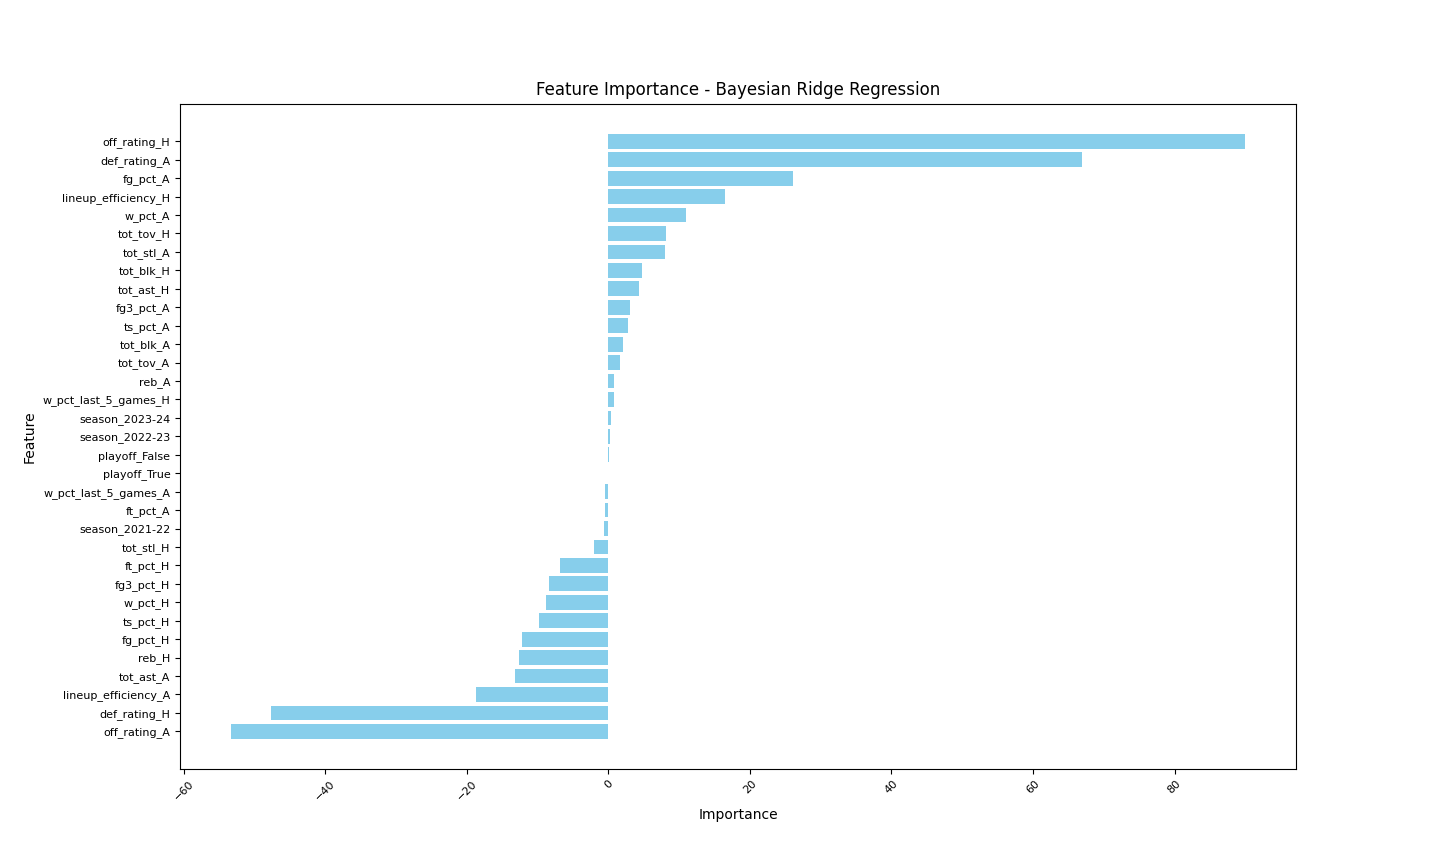
\includegraphics[width=\linewidth]{img/bayesian.png}
        \caption{Bayesian}
        \label{fig:first_label}
    \end{minipage}
    \hspace{0.05\linewidth}
    \begin{minipage}[b]{0.45\linewidth}
        \centering
        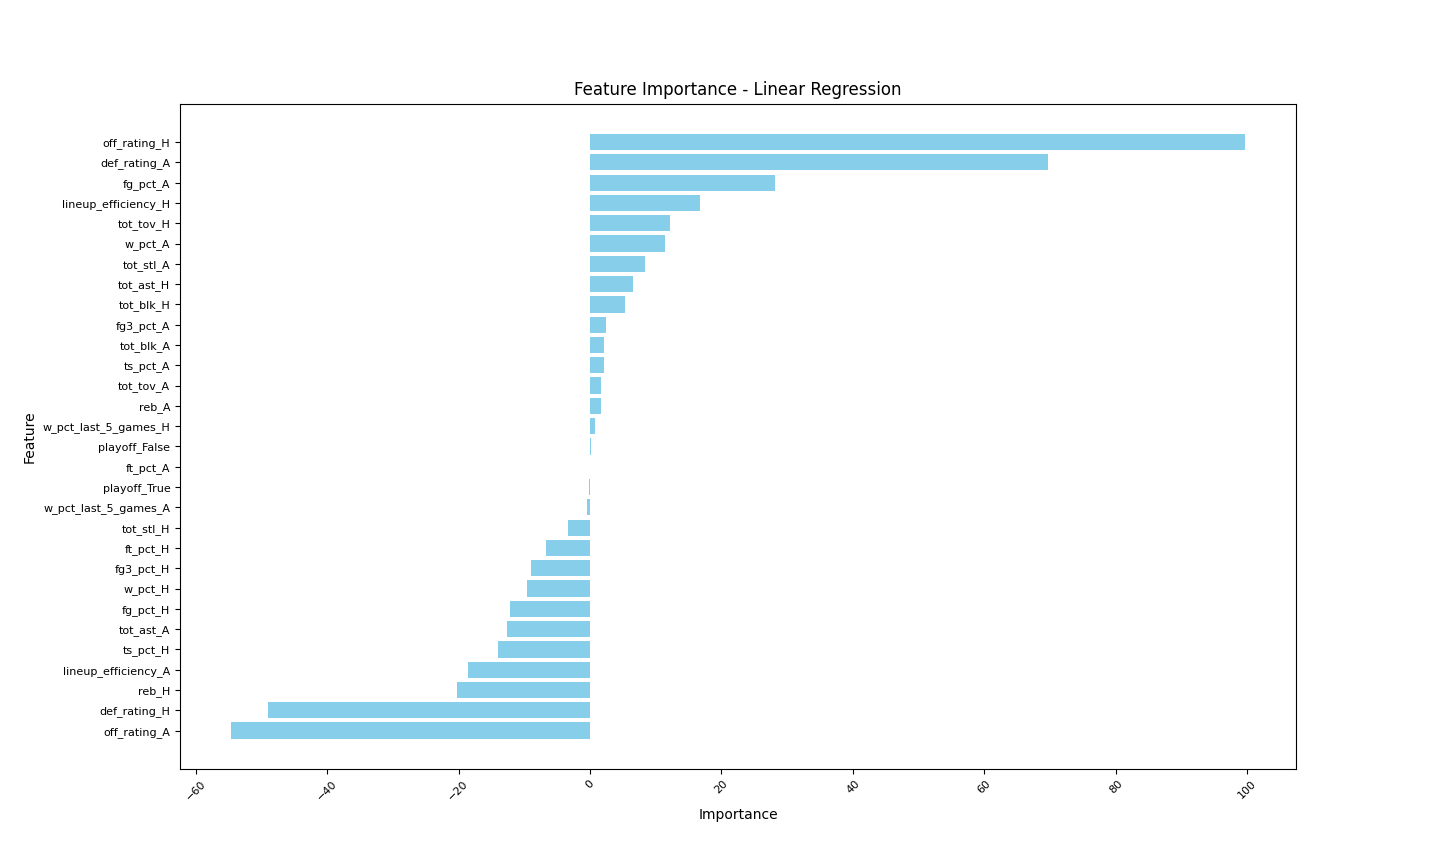
\includegraphics[width=\linewidth]{img/linear_regression.png}
        \caption{Linear Regression}
        \label{fig:second_label}
    \end{minipage}
\end{figure}

\begin{figure}[H]
    \centering
    \begin{minipage}[b]{0.45\linewidth}
        \centering
        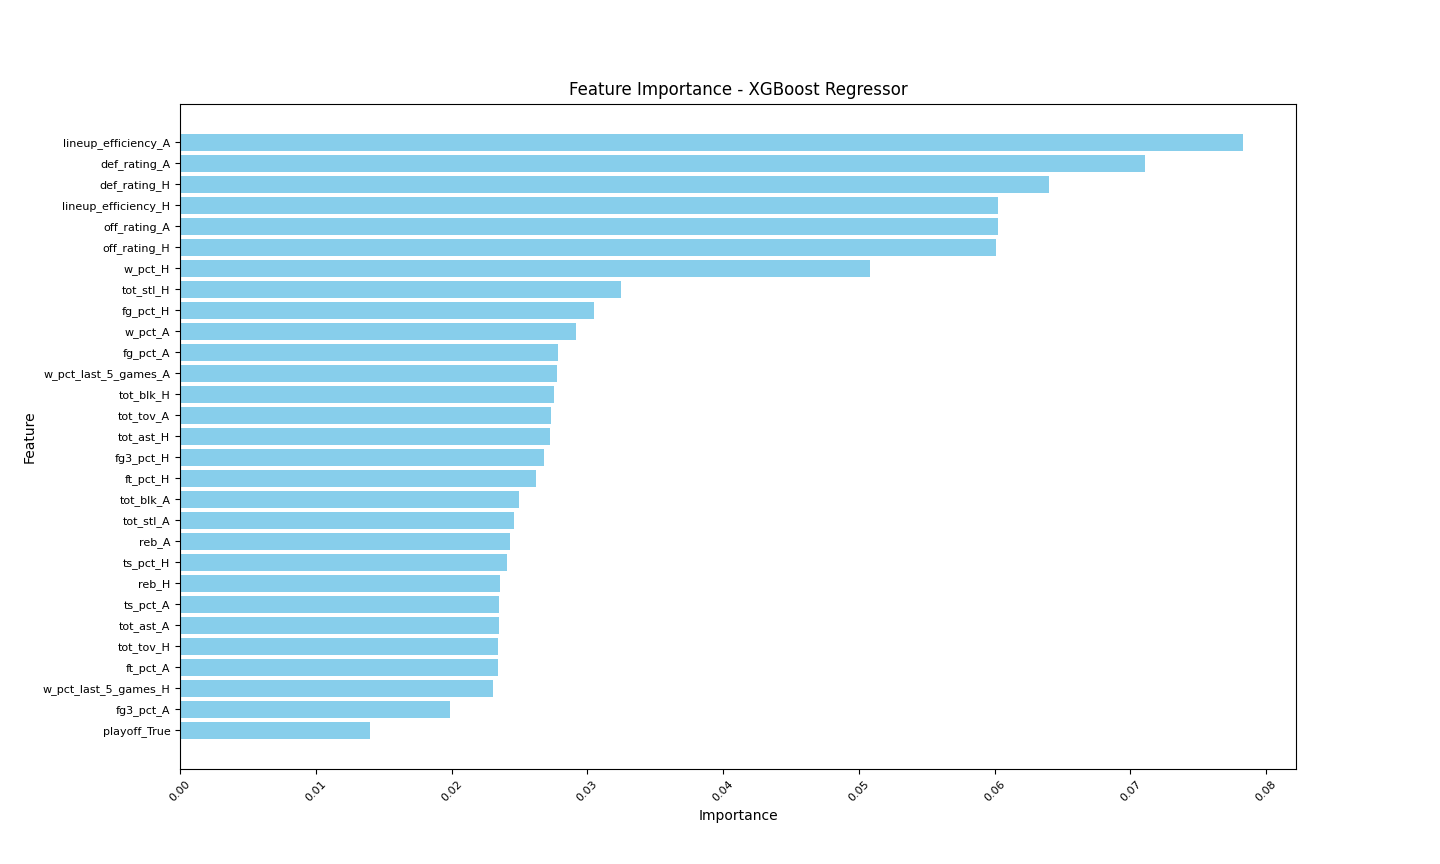
\includegraphics[width=\linewidth]{img/xgboost.png}
        \caption{XGBoost}
        \label{fig:first_label}
    \end{minipage}
    \hspace{0.05\linewidth}
    \begin{minipage}[b]{0.45\linewidth}
        \centering
        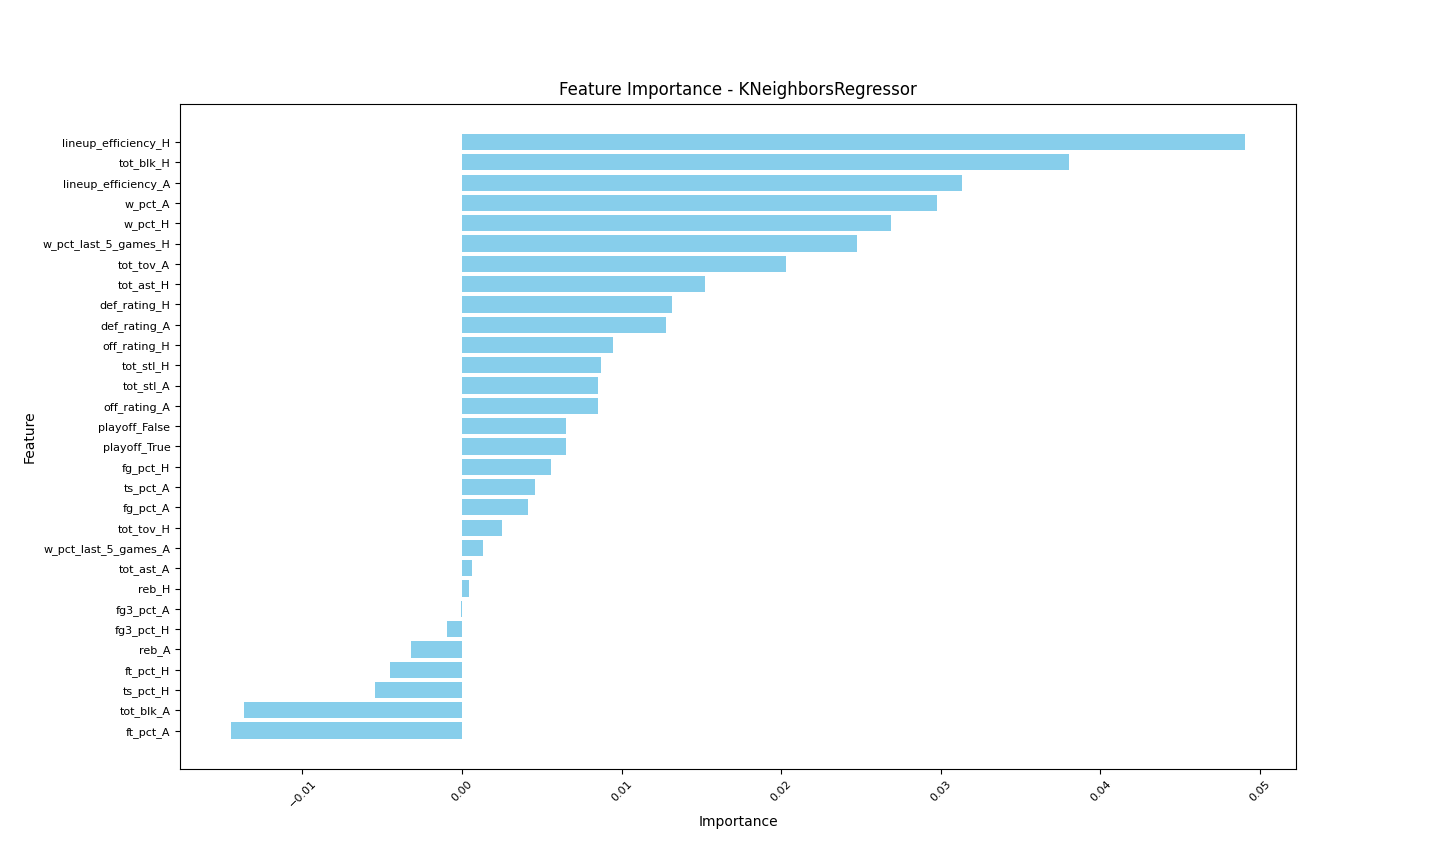
\includegraphics[width=\linewidth]{img/knn.png}
        \caption{K-Nearest Neighbors}
        \label{fig:second_label}
    \end{minipage}
\end{figure}

Si può vedere come i 3 modelli migliori (ovvero bayesian, xgboost e linear regression) valutino maggiormente, e dunque prediligano, le seguenti metriche:
\begin{itemize}
    \item lineup\_efficiency\_A
    \item lineup\_efficiency\_H
    \item off\_rating\_A
    \item off\_rating\_H
    \item def\_rating\_H
    \item def\_rating\_A
\end{itemize} 
Al contrario, il modello di regressione K-Nearest Neighbors mantiene solo le lineup\_efficiency ed altre features, a scapito di:
off\_rating\_A
off\_rating\_H
def\_rating\_A
def\_rating\_H

\newpage
